% Chapter 3: Design
% Main chapter title is set in main.tex via \chapter{Design}

\section{System Architecture}

The Hybrid Post-Quantum VPN system is designed as a secure client-gateway architecture that combines classical and post-quantum cryptographic primitives to establish a quantum-resistant encrypted tunnel over untrusted networks. The system consists of two major components: a client-side desktop controller with a local VPN agent and a remote gateway server responsible for authentication, key exchange, and encrypted packet forwarding.

The architecture follows a modular design approach to ensure scalability, maintainability, and cryptographic agility. The implementation integrates classical cryptography such as X25519 and ECDSA-P256 with post-quantum algorithms including ML-KEM-768 and ML-DSA.

\begin{figure}[H]
    \centering
    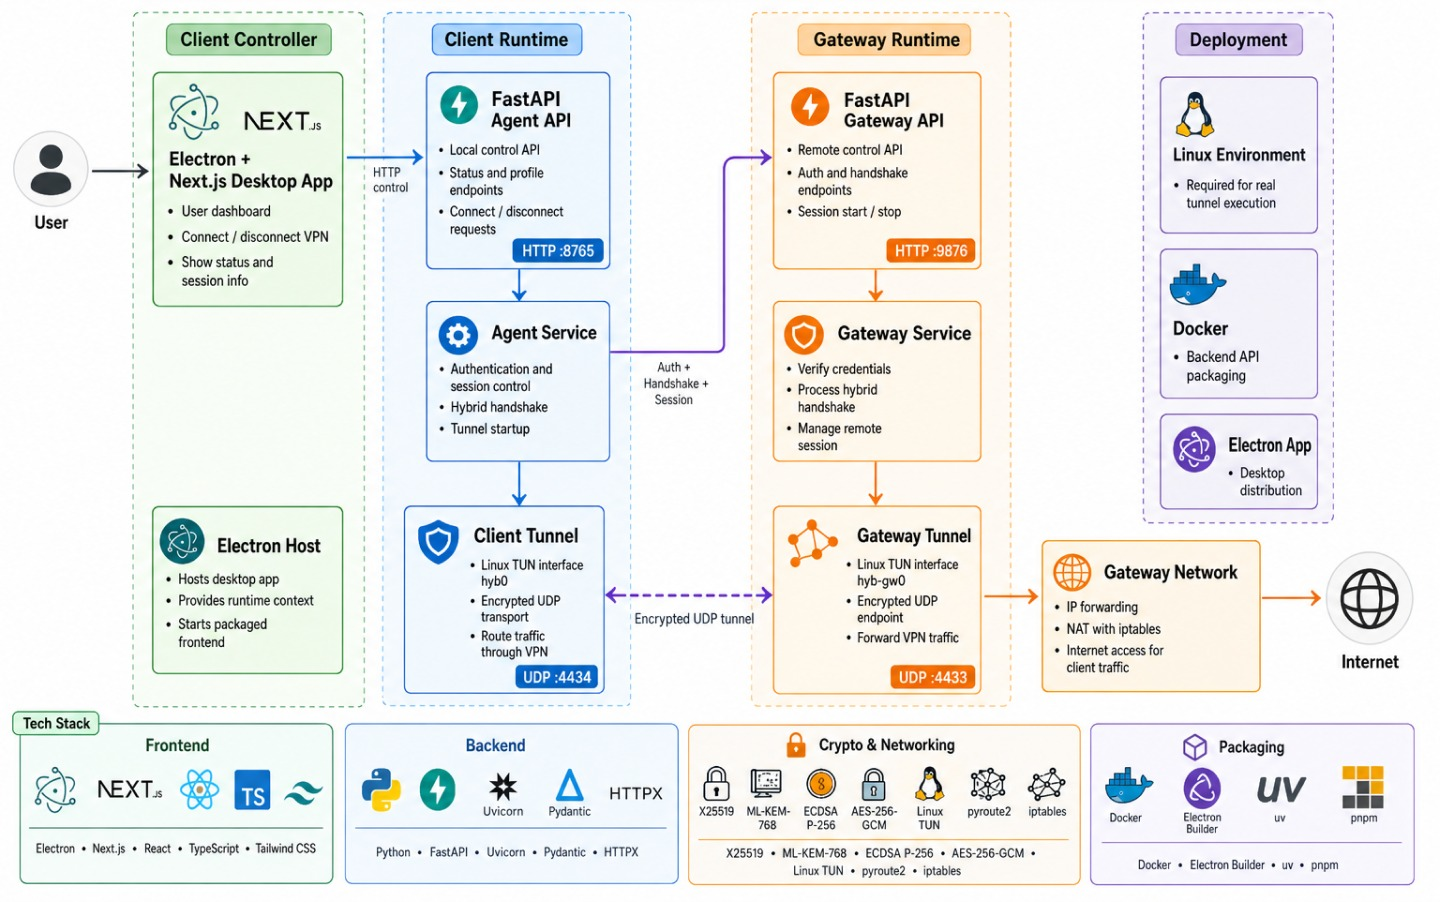
\includegraphics[width=\textwidth]{hybrid-vpn-architecture.jpeg}
    \caption{Architecture of the Hybrid Post-Quantum VPN System}
    \label{fig:system-architecture}
\end{figure}

\subsection{Client Node}

The client node consists of the following major components:

\begin{enumerate}
    \item \textbf{Electron + Next.js Desktop Dashboard}
    \begin{itemize}
        \item Provides a graphical user interface for initiating and managing VPN connections.
        \item Displays tunnel status, active cryptographic suite, throughput statistics, and connection logs.
        \item Communicates with the local Python Agent API through HTTP endpoints.
    \end{itemize}

    \item \textbf{Python Agent API}
    \begin{itemize}
        \item Handles authentication and handshake coordination with the gateway.
        \item Creates and manages the Linux TUN interface.
        \item Encrypts and decrypts packets using AES-256-GCM.
        \item Implements replay protection using sequence numbers and nonce tracking.
    \end{itemize}

    \item \textbf{TUN Interface}
    \begin{itemize}
        \item Creates a virtual Layer-3 network interface (\texttt{hyb0}).
        \item Captures outgoing IPv4 packets and forwards them through the encrypted UDP tunnel.
    \end{itemize}
\end{enumerate}

\subsection{Gateway Node}

The gateway node acts as the secure endpoint of the VPN tunnel.

\begin{enumerate}
    \item \textbf{Gateway API}
    \begin{itemize}
        \item Performs peer authentication and hybrid key exchange.
        \item Validates handshake requests and negotiates cryptographic algorithms.
        \item Manages secure session establishment.
    \end{itemize}

    \item \textbf{UDP Tunnel Service}
    \begin{itemize}
        \item Receives encrypted packets from the client.
        \item Performs AES-256-GCM authentication tag verification.
        \item Decrypts and forwards packets to the gateway TUN interface.
    \end{itemize}

    \item \textbf{Gateway TUN Interface}
    \begin{itemize}
        \item Creates the virtual interface \texttt{hyb-gw0}.
        \item Enables bidirectional forwarding between the secure tunnel and the target network.
    \end{itemize}
\end{enumerate}

\subsection{Hybrid Cryptographic Workflow}

The proposed VPN integrates both classical and post-quantum cryptographic operations during session establishment.

\begin{enumerate}
    \item \textbf{Classical Key Exchange}
    \begin{itemize}
        \item Uses X25519 Elliptic Curve Diffie-Hellman to derive a classical shared secret.
    \end{itemize}

    \item \textbf{Post-Quantum Key Encapsulation}
    \begin{itemize}
        \item Uses ML-KEM-768 to generate a post-quantum shared secret resistant to quantum attacks.
    \end{itemize}

    \item \textbf{Key Derivation}
    \begin{itemize}
        \item Both secrets are concatenated and processed using HKDF-SHA256 to derive the final session keys.
    \end{itemize}

    \item \textbf{Authentication}
    \begin{itemize}
        \item The current implementation uses ECDSA-P256 signatures.
        \item Future implementation includes hybrid authentication using ML-DSA.
    \end{itemize}

    \item \textbf{Data Encryption}
    \begin{itemize}
        \item Tunnel traffic is encrypted using AES-256-GCM with unique nonces and authentication tags.
    \end{itemize}
\end{enumerate}

\section{System Workflow}

The workflow of the Hybrid Post-Quantum VPN system consists of authentication, hybrid handshake establishment, secure tunnel creation, and encrypted packet forwarding.



\subsection{Connection Establishment}

\begin{enumerate}
    \item The client initiates a connection request from the Electron dashboard.
    
    \item The Agent API sends a handshake request to the gateway.
    
    \item The gateway negotiates supported algorithms:
    \begin{itemize}
        \item X25519
        \item ML-KEM-768
        \item AES-256-GCM
        \item HKDF-SHA256
    \end{itemize}

    \item Both parties perform:
    \begin{itemize}
        \item X25519 key exchange
        \item ML-KEM-768 encapsulation and decapsulation
    \end{itemize}

    \item The derived secrets are combined using HKDF-SHA256 to produce session keys.

    \item Mutual authentication is performed using digital signatures.

    \item Upon successful verification, Linux TUN interfaces are created on both systems.

    \item Secure encrypted communication begins over UDP.
\end{enumerate}

\subsection{Packet Processing}

\begin{enumerate}
    \item IPv4 packets are captured from the TUN interface.

    \item Packets are encrypted using AES-256-GCM.

    \item A sequence number and nonce are attached to each packet.

    \item The encrypted packet is transmitted through UDP sockets.

    \item The receiving endpoint verifies:
    \begin{itemize}
        \item Nonce validity
        \item Authentication tag integrity
        \item Replay protection sequence number
    \end{itemize}

    \item Valid packets are decrypted and forwarded to the destination TUN interface.
\end{enumerate}

\section{Technology Stack}

The project combines modern networking, cryptographic, and frontend technologies to implement a research-grade hybrid VPN prototype.

\begin{table}[H]
\centering
\caption{Technology Stack Used in the Hybrid VPN}
\begin{tabular}{|c|c|}
\hline
\textbf{Category} & \textbf{Technologies} \\
\hline
Frontend & Next.js, React, Tailwind CSS, Electron, TypeScript \\
\hline
Backend & Python, FastAPI, AsyncIO \\
\hline
Classical Cryptography & OpenSSL, X25519, ECDSA-P256, AES-256-GCM \\
\hline
Post-Quantum Cryptography & liboqs, ML-KEM-768, ML-DSA \\
\hline
Networking & Linux TUN/TAP, UDP Sockets, pyroute2 \\
\hline
Security & HKDF-SHA256, Replay Protection, Nonce Validation \\
\hline
Deployment & Docker, Ubuntu Linux Virtual Machines \\
\hline
Testing Tools & Wireshark, tcpdump, pytest \\
\hline
\end{tabular}
\label{tab:tech-stack}
\end{table}

\section{Module Design}

The system is divided into multiple functional modules for maintainability and extensibility.

\subsection{Cryptographic Module}

\begin{itemize}
    \item Implements X25519 key exchange.
    \item Integrates ML-KEM-768 using liboqs.
    \item Performs HKDF-SHA256 key derivation.
    \item Provides AES-256-GCM encryption and decryption.
\end{itemize}

\subsection{Tunnel Management Module}

\begin{itemize}
    \item Creates Linux TUN interfaces.
    \item Configures routing and IP addresses using pyroute2.
    \item Manages encrypted UDP forwarding.
\end{itemize}

\subsection{Authentication Module}

\begin{itemize}
    \item Performs ECDSA-P256 signature verification.
    \item Maintains handshake transcript validation.
    \item Supports future integration of ML-DSA hybrid authentication.
\end{itemize}

\subsection{Frontend Dashboard Module}

\begin{itemize}
    \item Displays tunnel status and performance metrics.
    \item Allows connect/disconnect operations.
    \item Provides browser-mode fallback during development.
\end{itemize}

\section{Security Design Considerations}

The proposed VPN incorporates several security mechanisms to ensure confidentiality, integrity, and resilience against future threats.

\begin{enumerate}
    \item \textbf{Hybrid Cryptography}
    \begin{itemize}
        \item Session security depends on both classical and post-quantum primitives.
    \end{itemize}

    \item \textbf{Forward Secrecy}
    \begin{itemize}
        \item Ephemeral X25519 keys ensure compromise of long-term keys does not expose previous sessions.
    \end{itemize}

    \item \textbf{Replay Protection}
    \begin{itemize}
        \item Sequence numbers and nonce validation prevent replay attacks.
    \end{itemize}

    \item \textbf{Authenticated Encryption}
    \begin{itemize}
        \item AES-256-GCM ensures confidentiality and packet integrity simultaneously.
    \end{itemize}

    \item \textbf{Transcript Binding}
    \begin{itemize}
        \item HKDF derivation incorporates handshake transcript hashes to prevent downgrade attacks.
    \end{itemize}

    \item \textbf{Cryptographic Agility}
    \begin{itemize}
        \item Modular design allows replacement of PQC algorithms in future versions.
    \end{itemize}
\end{enumerate}

\section{Deployment Design}

The prototype is designed primarily for Linux-based virtual machine deployment.

\subsection{Virtual Machine Setup}

\begin{itemize}
    \item VM 1 acts as the client system.
    \item VM 2 acts as the gateway server.
    \item Ubuntu 22.04/24.04 is used as the operating system.
    \item Bridged networking is preferred for direct VM-to-VM communication.
\end{itemize}

\subsection{Docker Deployment}

The backend services can also be deployed using Docker containers.

\begin{itemize}
    \item Containers expose:
    \begin{itemize}
        \item Agent API port 8765
        \item Gateway API port 9876
        \item UDP tunnel ports 4433 and 4434
    \end{itemize}

    \item Linux capabilities:
    \begin{itemize}
        \item \texttt{NET\_ADMIN}
        \item Access to \texttt{/dev/net/tun}
    \end{itemize}
    are required for TUN interface creation inside containers.
\end{itemize}